\documentclass[a4paper]{article} 
\addtolength{\hoffset}{-2.25cm}
\addtolength{\textwidth}{4.5cm}
\addtolength{\voffset}{-3.25cm}
\addtolength{\textheight}{5cm}
\setlength{\parskip}{0pt}
\setlength{\parindent}{0in}

%----------------------------------------------------------------------------------------
%	PACKAGES AND OTHER DOCUMENT CONFIGURATIONS
%----------------------------------------------------------------------------------------

\usepackage[italicdiff]{physics}
%\usepackage{derivative}
\usepackage{tasks}
\usepackage{blindtext} % Package to generate dummy text
\usepackage{charter} % Use the Charter font
\usepackage[utf8]{inputenc} % Use UTF-8 encoding
\usepackage{microtype} % Slightly tweak font spacing for aesthetics
\usepackage[T1]{fontenc}
\usepackage{polski}
\usepackage{enumerate}
\usepackage[utf8]{inputenc}
\usepackage[english, ngerman]{babel} % Language hyphenation and typographical rules
\usepackage{amsthm, amsmath, amssymb} % Mathematical typesetting
\usepackage{float} % Improved interface for floating objects
\usepackage[final, colorlinks = true, 
            linkcolor = black, 
            citecolor = black]{hyperref} % For hyperlinks in the PDF
\usepackage{graphicx, multicol} % Enhanced support for graphics
\usepackage{xcolor} % Driver-independent color extensions
\usepackage{marvosym, wasysym} % More symbols
\usepackage{rotating} % Rotation tools
\usepackage{censor} % Facilities for controlling restricted text
\usepackage{listings, style/lstlisting} % Environment for non-formatted code, !uses style file!
\usepackage{pseudocode} % Environment for specifying algorithms in a natural way
\usepackage{style/avm} % Environment for f-structures, !uses style file!
\usepackage{booktabs} % Enhances quality of tables
\usepackage{tikz-qtree} % Easy tree drawing tool
\tikzset{every tree node/.style={align=center,anchor=north},
         level distance=2cm} % Configuration for q-trees
\usepackage{style/btree} % Configuration for b-trees and b+-trees, !uses style file!
\usepackage[backend=biber,style=numeric,
            sorting=nyt]{biblatex} % Complete reimplementation of bibliographic facilities
\addbibresource{ecl.bib}
\usepackage{csquotes} % Context sensitive quotation facilities
\usepackage[yyyymmdd]{datetime} % Uses YEAR-MONTH-DAY format for dates
\renewcommand{\dateseparator}{-} % Sets dateseparator to '-'
\usepackage{fancyhdr} % Headers and footers
\pagestyle{fancy} % All pages have headers and footers
\fancyhead{}\renewcommand{\headrulewidth}{0pt} % Blank out the default header
\fancyfoot[L]{} % Custom footer text
\fancyfoot[C]{} % Custom footer text
\fancyfoot[R]{\thepage} % Custom footer text
\newcommand{\note}[1]{\marginpar{\scriptsize \textcolor{red}{#1}}} %
\graphicspath{ {./images/} }

%----------------------------------------------------------------------------------------

\begin{document}

%-------------------------------
%	TITLE SECTION
%-------------------------------

\fancyhead[C]{}
\hrule \medskip % Upper rule
\begin{minipage}{0.295\textwidth} 
\raggedright
\footnotesize
Antoni Dąbrowski \hfill\\   
Nr. indeksu 317214\hfill\\
Mail: 317214@uwr.edu.pl
\end{minipage}
\begin{minipage}{0.4\textwidth} 
\centering 
\large 
Sieci komputerowe\\ 
\normalsize 
Ćwiczenia - lista I\\ 
\end{minipage}
\begin{minipage}{0.295\textwidth} 
\raggedleft
\today\hfill\\
\end{minipage}
\medskip\hrule 
\bigskip

%-------------------------------
%	CONTENTS
%-------------------------------

\begin{center}
\begin{tabular}{ |c|c|c|c|c|c|c|c|c|c| } 
 \hline
 1 & 2 & 3 & 4 & 5 & 6 & 7 & 8 & 9 & 10 \\ 
 \hline
 \checkmark & \checkmark & \checkmark & \checkmark & \checkmark & \checkmark & \checkmark & \checkmark &  &  \\ 
 \hline
\end{tabular}
\end{center}



\section{Zadanie pierwsze}
Dla każdego z podanych poniżej adresów IP w notacji CIDR określ, czy jest to adres sieci, adres rozgłoszeniowy czy też adres komputera. W każdym przypadku wyznacz odpowiadający mu adres sieci, rozgłoszeniowy i jakiś adres IP innego komputera w tej samej sieci.
\begin{itemize}
\item 10.1.2.3/8
\item 156.17.0.0/16
\item 99.99.99.99/27
\item 156.17.64.4/30
\item 123.123.123.123/32
\end{itemize}

\subsection{Rozwiązanie}
Classless Inter-Domain Routing (CIDR) – bezklasowa metoda przydzielania adresów IP. CIDR wykorzystuje maskę podsieci do ustalenia zmiennej części 32-bitowego adresu IP sieci. Adres sieciowy jest zawsze pierwszym, natomiast adres rozgłoszeniowy jest zawsze ostatnim spośród klasy adresów definiowanych przez dany adres i maskę. Pozostałe dostępne adresy są adresami komputerów.
\begin{itemize}
\item $10.1.2.3/8\rightarrow00001010|.00000001.0000001000000011$ - adres komputera\\
$00001010|.00000000.00000000.0000000$ - adres sieci\\
$00001010|.11111111.11111111.11111111$ - adres rozgłoszeniowy
\item $156.17.0.0/16\rightarrow10011100.00010001|00000000.00000000$ - adres sieci\\
$10011100.00010001|00000000.00000001$ - adres komputera\\
$10011100.00010001|11111111.11111111$ - adres rozgłoszeniowy
\item $99.99.99.99/27\rightarrow01100011.01100011.01100011.011|00011$ - adres komputera\\
$01100011.01100011.01100011.011|00000$ - adres sieci\\
$01100011.01100011.01100011.011|11111$ - adres rozgłoszeniowy
\item $156.17.64.4/30\rightarrow10011100.00010001.01000000.000001|00$ - adres sieci\\
$10011100.00010001.01000000.000001|01$ - adres komputera\\
$10011100.00010001.01000000.000001|11$ - adres rozgłoszeniowy
\item $123.123.123.123/32\rightarrow01111011.01111011.01111011.01111011|$ - adres komputera\\
W przypadku maski 32-bitowej jedynym adresem jest adres urządzenia. W szczególności nie ma adresu rozgłoszeniowego ani adresu sieci.
\end{itemize}

%------------------------------------------------

\section{Zadanie drugie}
Podziel sieć 10.10.0.0/16 na 5 rozłącznych podsieci, tak aby każdy z adresów IP z sieci 10.10.0.0/16 był w jednej z tych 5 podsieci. Jak zmieniła się liczba adresów IP możliwych do użycia przy adresowaniu komputerów? Jaki jest minimalny rozmiar podsieci, który możesz uzyskać w ten sposób?

\subsection{Rozwiązanie}
Podział:\\
00001010.00001010.10000000.00000000/17\\
00001010.00001010.00000000.00000000/19\\
00001010.00001010.00100000.00000000/19\\
00001010.00001010.01000000.00000000/19\\
00001010.00001010.01100000.00000000/19\\

Zmiana liczy możliwych do użycia adresów IP:\\
Było $2^{16}-2$, jest $2^{16}-2\cdot5$.\\

Minimalny rozmiar podsieci:\\
Chcemy, aby podział był na rozłączne zbiory, dające w sumie (mnogościowej) wszystkie adresy kodowane przez podany adres i maskę 16-bitową. Rozważmy prostszy problem - podział na dwie rozłączne podsieci. Tu widać wprost, że jedyną opcją jest podział na $$00001010.00001010.00000000.00000000/17$$ $$00001010.00001010.10000000.00000000/17$$\\
Dla podziału na trzy sieci, problem sprowadza się do rozstrzygnięcia, którą z stworzonych uprzednio dwóch sieci podzielić na pół. Idąc tym tokiem rozumowania dalej możemy stwierdzić, że uzyskanie najmniejszej podsieci może nastąpić jedynie, gdy zastosujemy następujący algorytm. Jeżeli osiągnąłem oczekiwaną liczbę podziałów zakończ, wpp podziel adres, wybierz jeden z podzielonych i odpal na nim ten algorytm. W tym przypadku:\\


00001010.00001010.00000000.00000000/17\\
00001010.00001010.10000000.00000000/18\\
00001010.00001010.11000000.00000000/19\\
00001010.00001010.11100000.00000000/20\\
00001010.00001010.11110000.00000000/20\\

Najmniejsza podsiećsieć ma $2^{12}$ adresów.

%------------------------------------------------

\section{Zadanie trzecie}
Tablica routingu zawiera następujące wpisy (podsieć → dokąd wysłać):
\begin{itemize}
\item 0.0.0.0/0 → do routera A
\item 10.0.0.0/23 → do routera B
\item 10.0.2.0/24 → do routera B
\item 10.0.3.0/24 → do routera B
\item 10.0.1.0/24 → do routera C
\item 10.0.0.128/25 → do routera B
\item 10.0.1.8/29 → do routera B
\item 10.0.1.16/29 → do routera B
\item 10.0.1.24/29 → do routera B
\end{itemize}
Napisz równoważną tablicę routingu zawierającą jak najmniej wpisów.


\subsection{Rozwiązanie}
Dane:
\begin{center}
\begin{tabular}{ |c|c|c| } 
 \hline
 0.0.0.0/0 & |00000000.00000000.00000000.00000000 & routera A \\ 
 10.0.0.0/23 & 00001010.00000000.0000000|0.00000000 & routera B \\ 
 10.0.2.0/24 & 00001010.00000000.00000010|.00000000 & routera B \\
10.0.3.0/24 & 00001010.00000000.00000011|.00000000 & routera B \\
10.0.1.0/24 & 00001010.00000000.00000001|.00000000 & routera C \\
10.0.0.128/25 & 00001010.00000000.00000000.1|0000000 & routera B\\
10.0.1.8/29 & 00001010.00000000.00000001.00001|000 & routera B\\
10.0.1.16/29 & 00001010.00000000.00000001.00010|000 & routera B\\
10.0.1.24/29 & 00001010.00000000.00000001.00011|000 & routera B\\
 \hline
\end{tabular}
\end{center}
Skrócona tablica routingu:
\begin{center}
\begin{tabular}{ |c|c|c| } 
 \hline
 0.0.0.0/0 & |00000000.00000000.00000000.00000000 & routera A \\ 
 10.0.0.0/22 & 00001010.00000000.0000000|0.00000000 & routera B \\ 
10.0.1.0/24 & 00001010.00000000.00000001|.00000000 & routera C \\
10.0.1.0/27 & 00001010.00000000.00000001.000|00000 & routera B\\
10.0.1.0/29 & 00001010.00000000.00000001.00000|000 & routera C\\
 \hline
\end{tabular}
\end{center}


%------------------------------------------------

\section{Zadanie czwarte}
Wykonaj powyższe zadanie dla tablicy
\begin{itemize}
\item 0.0.0.0/0 → do routera A
\item 10.0.0.0/8 → do routera B
\item 10.3.0.0/24 → do routera C
\item 10.3.0.32/27 → do routera B
\item 10.3.0.64/27 → do routera B
\item 10.3.0.96/27 → do routera B
\end{itemize}
Napisz równoważną tablicę routingu zawierającą jak najmniej wpisów.


\subsection{Rozwiązanie}
Dane:
\begin{center}
\begin{tabular}{ |c|c|c| } 
 \hline
 0.0.0.0/0 & |00000000.00000000.00000000.00000000 & routera A \\ 
 10.0.0.0/8 & 00001010|.00000000.00000000.00000000 & routera B \\ 
10.3.0.0/24 & 00001010.00000011.00000000|.00000000 & routera C \\
10.3.0.32/27 & 00001010.00000011.00000000.001|00000 & routera B\\
10.3.0.64/27 & 00001010.00000011.00000000.010|00000 & routera B\\
10.3.0.96/27 & 00001010.00000011.00000000.011|00000 & routera B\\
 \hline
\end{tabular}
\end{center}
Skrócona tablica routingu:
\begin{center}
\begin{tabular}{ |c|c|c| } 
 \hline
 0.0.0.0/0 & |00000000.00000000.00000000.00000000 & routera A \\ 
 10.0.0.0/8 & 00001010|.00000000.00000000.00000000 & routera B \\ 
10.3.0.0/24 & 00001010.00000011.00000000|.00000000 & routera C \\
10.3.0.64/26 & 00001010.00000011.00000000.01|000000 & routera B\\
10.3.0.32/27 & 00001010.00000011.00000000.001|00000 & routera B\\
 \hline
\end{tabular}
\end{center}
%------------------------------------------------
\section{Zadanie piąte}
Jak uporządkować wpisy w tablicy routingu, żeby zasada najlepszego dopasowania odpowiadała wyborowi „pierwszy pasujący” (tj. przeglądaniu tablicy od początku do końca aż do momentu napotkania dowolnej pasującej reguły)? Odpowiedź uzasadnij formalnie.

\subsection{Rozwiązanie}
Wystarczy uporządkować adresy od najbardziej szczegółowych, do najbardziej ogólnych, tj. malejąco po długości maski.\\

Uzasadnienie:\\
Załóżmy nie wprost, że stosując zaproponowaną przeze mnie kolejność pewien adres został wysłany do routera B, pomimo że powinien trafić do routera A.  \\

Adres powinien trafić do routera A $\implies$ spośród wszystkich grup adresów w notacji CIDR pasujących do danego adresu tan o najdłuższej masce kierował do routera A.\\

Adres trafił do routera B $\implies$ pierwsza (w kolejności malejącej po długości masek) grupa adresów w notacji CIDR pasująca do danego adresu kierowała go do routera B\\

Zatem w tablicy routingu istnieją dwa wpisy opisujące dokładnie tę samą grupę adresów oraz kierują do innych routerów, co jest w sprzeczności z działaniem tablic routingu.

%------------------------------------------------

\section{Zadanie szóste}
W podanej niżej sieci tablice routingu budowane są za pomocą algorytmu wektora odległości. Pokaż (krok po kroku), jak będzie się to odbywać. W ilu krokach zostanie osiągnięty stan stabilny?

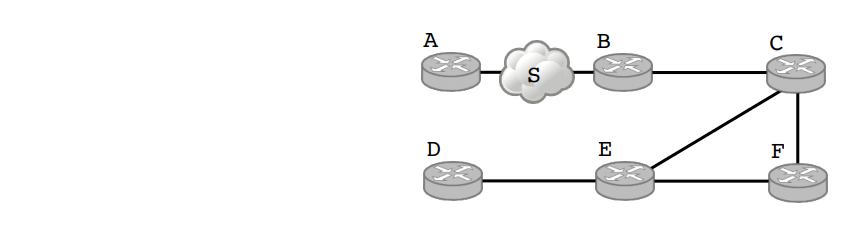
\includegraphics{Zadanie_szóste}

\subsection{Rozwiązanie}
\begin{center}
\begin{tabular}{ |c|c|c|c|c|c|c| } 
 \hline
 tablica\textbackslash router & A & B & C & D & E & F \\ 
 \hline
 trasa do A & - & 1 & $\infty$ & $\infty$ & $\infty$ & $\infty$  \\ 
 \hline
 trasa do B & 1 & - & 1 & $\infty$ & $\infty$ & $\infty$ \\ 
 \hline
 trasa do C & $\infty$ & 1 & - & $\infty$ & 1 & 1 \\ 
 \hline
 trasa do D & $\infty$ & $\infty$ & $\infty$ & - & 1 & $\infty$ \\ 
 \hline
 trasa do E & $\infty$ & $\infty$ & 1 & 1 & - & 1 \\ 
 \hline
 trasa do F & $\infty$ & $\infty$ & 1 & $\infty$ & 1 & - \\ 
 \hline
 trasa do S & 1 & 1 & $\infty$ & $\infty$ & $\infty$ & $\infty$ \\ 
 \hline
\end{tabular}
\end{center}

\begin{center}
\begin{tabular}{ |c|c|c|c|c|c|c| } 
 \hline
 tablica\textbackslash router & A & B & C & D & E & F \\ 
 \hline
 trasa do A & - & 1 & \textbf{2 (via B)} & $\infty$ & $\infty$ & $\infty$  \\ 
 \hline
 trasa do B & 1 & - & 1 & $\infty$ & \textbf{2 (via C)} & \textbf{2 (via C)} \\ 
 \hline
 trasa do C & 2 \textbf{(via B)} & 1 & - & \textbf{2 (via E)} & 1 & 1 \\ 
 \hline
 trasa do D & $\infty$ & $\infty$ & \textbf{2 (via E)} & - & 1 & \textbf{2 (via E)} \\ 
 \hline
 trasa do E & $\infty$ & \textbf{2 (via C)} & 1 & 1 & - & 1 \\ 
 \hline
 trasa do F & $\infty$ & \textbf{2 (via C)} & 1 & \textbf{2 (via E)} & 1 & - \\ 
 \hline
 trasa do S & 1 & 1 & \textbf{2 (via B)} & $\infty$ & $\infty$ & $\infty$ \\ 
 \hline
\end{tabular}
\end{center}

\begin{center}
\begin{tabular}{ |c|c|c|c|c|c|c| } 
 \hline
 tablica\textbackslash router & A & B & C & D & E & F \\ 
 \hline
 trasa do A & - & 1 & 2 (via B) & $\infty$ & \textbf{3 (via C)} & \textbf{3 (via C)}  \\ 
 \hline
 trasa do B & 1 & - & 1 & \textbf{3 (via E)} & 2 (via C) & 2 (via C) \\ 
 \hline
 trasa do C & 2 (via B) & 1 & - & 2 (via E) & 1 & 1 \\ 
 \hline
 trasa do D & $\infty$ & \textbf{3 (via C)} & 2 (via E) & - & 1 & 2 (via E) \\ 
 \hline
 trasa do E & \textbf{3 (via B)} & 2 (via C) & 1 & 1 & - & 1 \\ 
 \hline
 trasa do F & \textbf{3 (via B)} & 2 (via C) & 1 & 2 (via E) & 1 & - \\ 
 \hline
 trasa do S & 1 & 1 & 2 (via B) & $\infty$ & \textbf{3 (via C)} & \textbf{3 (via C)} \\ 
 \hline
\end{tabular}
\end{center}

\begin{center}
\begin{tabular}{ |c|c|c|c|c|c|c| } 
 \hline
 tablica\textbackslash router & A & B & C & D & E & F \\ 
 \hline
 trasa do A & - & 1 & 2 (via B) & \textbf{4 (via E)} & 3 (via C) & 3 (via C)  \\ 
 \hline
 trasa do B & 1 & - & 1 & 3 (via E) & 2 (via C) & 2 (via C) \\ 
 \hline
 trasa do C & 2 (via B) & 1 & - & 2 (via E) & 1 & 1 \\ 
 \hline
 trasa do D & \textbf{4 (via B)} & 3 (via C) & 2 (via E) & - & 1 & 2 (via E) \\ 
 \hline
 trasa do E & 3 (via B) & 2 (via C) & 1 & 1 & - & 1 \\ 
 \hline
 trasa do F & 3 (via B) & 2 (via C) & 1 & 2 (via E) & 1 & - \\ 
 \hline
 trasa do S & 1 & 1 & 2 (via B) & \textbf{4 (via E)} & 3 (via C) & 3 (via C) \\ 
 \hline
\end{tabular}
\end{center}

%------------------------------------------------

\section{Zadanie siódme}
Załóżmy, że w powyższej sieci tablice routingu zostały już zbudowane. Co będzie się działo, jeśli zostanie dodane połączenie między routerami A i D?\\
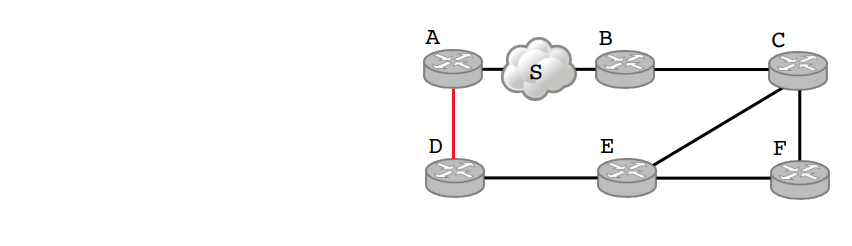
\includegraphics{Zadanie_siódme}
\subsection{Rozwiązanie}

\begin{center}
\begin{tabular}{ |c|c|c|c|c|c|c| } 
 \hline
 tablica\textbackslash router & A & B & C & D & E & F \\ 
 \hline
 trasa do A & - & 1 & 2 (via B) & \textbf{1} & 3 (via C) & 3 (via C)  \\ 
 \hline
 trasa do B & 1 & - & 1 & 3 (via E) & 2 (via C) & 2 (via C) \\ 
 \hline
 trasa do C & 2 (via B) & 1 & - & 2 (via E) & 1 & 1 \\ 
 \hline
 trasa do D & \textbf{1} & 3 (via C) & 2 (via E) & - & 1 & 2 (via E) \\ 
 \hline
 trasa do E & 3 (via B) & 2 (via C) & 1 & 1 & - & 1 \\ 
 \hline
 trasa do F & 3 (via B) & 2 (via C) & 1 & 2 (via E) & 1 & - \\ 
 \hline
 trasa do S & 1 & 1 & 2 (via B) & 4 (via E) & 3 (via C) & 3 (via C) \\ 
 \hline
\end{tabular}
\end{center}

\begin{center}
\begin{tabular}{ |c|c|c|c|c|c|c| } 
 \hline
 tablica\textbackslash router & A & B & C & D & E & F \\ 
 \hline
 trasa do A & - & 1 & 2 (via B) & 1 & \textbf{2 (via D)} & 3 (via C)  \\ 
 \hline
 trasa do B & 1 & - & 1 & \textbf{2 (via A)} & 2 (via C) & 2 (via C) \\ 
 \hline
 trasa do C & 2 (via B) & 1 & - & 2 (via E) & 1 & 1 \\ 
 \hline
 trasa do D & 1 & \textbf{2 (via A)} & 2 (via E) & - & 1 & 2 (via E) \\ 
 \hline
 trasa do E & \textbf{2 (via D)} & 2 (via C) & 1 & 1 & - & 1 \\ 
 \hline
 trasa do F & 3 (via B) & 2 (via C) & 1 & 2 (via E) & 1 & - \\ 
 \hline
 trasa do S & 1 & 1 & 2 (via B) & \textbf{2 (via A)} & 3 (via C) & 3 (via C) \\ 
 \hline
\end{tabular}
\end{center}


%------------------------------------------------
\section{Zadanie ósme}
W przedstawionej poniżej sieci uszkodzeniu ulega połączenie między routerami D i E. Załóżmy, że w sieci działa algorytm wektora odległości wykorzystujący technikę zatruwania ścieżki zwrotnej (poison reverse). Pokaż — opisując krok po kroku jakie komunikaty są przesyłane między routerami — że może powstać cykl w routingu.\\
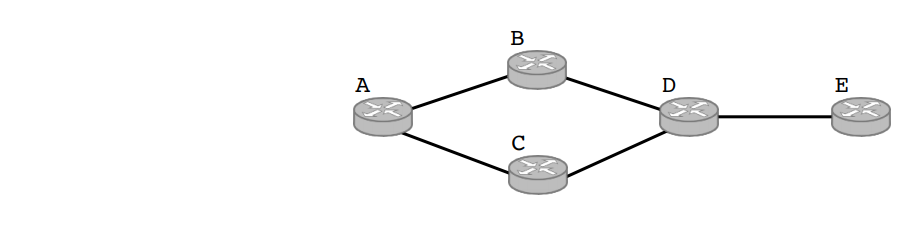
\includegraphics{Zadanie_ósme}

\subsection{Rozwiązanie}
Rozpatrzmy następujący scenariusz: 
\begin{itemize}
\item Krok 1: psuje się połączenie między routerem D i E.
\item Krok 2: informacja o tym zostaje przekazana do routerów B i C. Z jakiś powodów informacja idzie do routera C dużo dłużej niż do B.
\item Krok 3: router B otrzymując informację o zepsuciu ścieżki przekazuje tę informację do A. Wszystkie routery poza C mają w tym momencie nieskończone długości ścieżek do E.
\item Krok 4: nagle budzi się C i wysyła informację do sąsiedniych routerów, że może dojść do E ścieżką o długości 2.
\item Krok 5: routery A i B dostają informację o ścieżce do E prowadzącej przez A
\item Kolejne kroki cyklicznie powtarzają ostatnie dwa.
\end{itemize}

\begin{center}
\begin{tabular}{ |c|c|c|c|c| } 
 \hline
 \textbf{trasa do E\textbackslash router} & \textbf{A} & \textbf{B} & \textbf{C} & \textbf{D} \\ 
 \hline
 stan początkowy & 3 (via B) & 2 (via D) & 2 (via D) & 1 \\ 
 \hline
 krok 1 & 3 (via B) & 2 (via D) & 2 (via D) & $\infty$ \\ 
 \hline
 krok 2 & 3 (via B) & $\infty$ & 2 (via D) & $\infty$ \\ 
 \hline
 krok 3 & $\infty$ & $\infty$ & 2 (via D) & $\infty$ \\ 
 \hline
 krok 4 & 3 (via C) & $\infty$ & $\infty$ & 3 (via C) \\ 
 \hline
 krok 5 & $\infty$ & 4 (via A) & 4 (via A) & $\infty$ \\ 
 \hline
 $\vdots$ & $\vdots$ & $\vdots$ & $\vdots$ & $\vdots$ \\ 
 \hline
 krok $2n$ & $2n - 1$ (via C) & $\infty$ & $\infty$ & $2n - 1$ (via C) \\ 
 \hline
 krok $2n + 1$ & $\infty$ & $2n$ (via A) & $2n$ (via A) & $\infty$ \\ 
 \hline
\end{tabular}
\end{center}


%------------------------------------------------




\end{document}
